\documentclass[12pt]{article}
\usepackage[margin=1.0in]{geometry}
\usepackage{graphicx}
\usepackage[pdftex]{hyperref}
\usepackage{wrapfig}
\usepackage{float}
\usepackage{enumitem}
\usepackage{textcomp}
\usepackage[english]{babel}
\usepackage{csquotes}
\MakeOuterQuote{"}

\let\supscr=\textsuperscript

\begin{document}
\begin{titlepage}
    \centering
    \vspace{15cm}
    {\huge\bfseries Subsystems Report \par}
    \vspace{1cm}
    {\scshape\Large Jonathan "Sumner" Evans\par}
    \vfill
    {\scshape\large Section U\par}
    {\large \today\par}
    \vfill
\end{titlepage}

\section{Introduction}
A food desert is an area where access to fruits and vegetables is limited, too expensive, or
nonexistent due to a lack of grocery stores and farmers markets in a convenient walking distance.
\cite{cdc-food-deserts} People living in food deserts often rely on fringe food retailers and
discount stores for food. These retailers tend to sell high-fat and processed foods which
contributes to higher rates of obesity and diabetes in those food desert areas. According to the US
Department of Agriculture, there is a food desert in the Wheat Ridge area located between Wadsworth,
32\supscr{nd} Avenue, and 38\supscr{th} Avenue \cite{usda-food-deserts}.

The team’s goal is to empower English and Spanish speaking Wheat Ridge residents over 65 years in
age who live in food deserts and rely on food stamps to utilize a self-sustaining plant growing
system. Most of the system will come prepackaged for safe installation and use and will partially
use materials that can be sourced in the Wheat Ridge neighborhood. The net cost will be neutral or
better after two years of plant harvest and will include features that consider the potential
physical limitations of the stakeholders.

\section{Solution Description}
The team’s design solves the problem with five connected subsystems. A structural subsystem, a
reservoir and pump subsystem, a nutrient subsystem, a water delivery subsystem, and a hydroponic
bottle subsystem. The structural subsystem is compact, lightweight, and cost-effective. It uses a
three-step design which provides optimal growing space while allowing for compact storage in a $36"
\times 10" \times 24"$ area. The reservoir system is integrated into the structural subsystem and
consists of four separate water tanks. Each of these tanks corresponds to one growing stage and will
hold the nutrients necessary for that growing stage. The nutrient subsystem is housed partially
within the reservoir. It contains the nutrients necessary for each growing stage. Additionally it
provides instructions for caring for the plants. Nutrients are placed directly into the reservoirs.
Water and nutrients are distributed to each plant via the water delivery system. The water delivery
system distributes water and nutrients to each plant by pumping the water to the top row and
allowing the water to flow to each consecutive bottle by the force of gravity. The hydroponic bottle
subsystem is made of re-purposed 2-litre soda bottles. The final solution includes an easy-to-use
tool allowing stakeholders to make the bottles themselves.

\section{Subsystem Description}

\section{Subsystem Interfaces}

\section{Subsystem Analysis}

\section{Summary}

\pagebreak
%\begin{figure}[H]
%    \centering
%    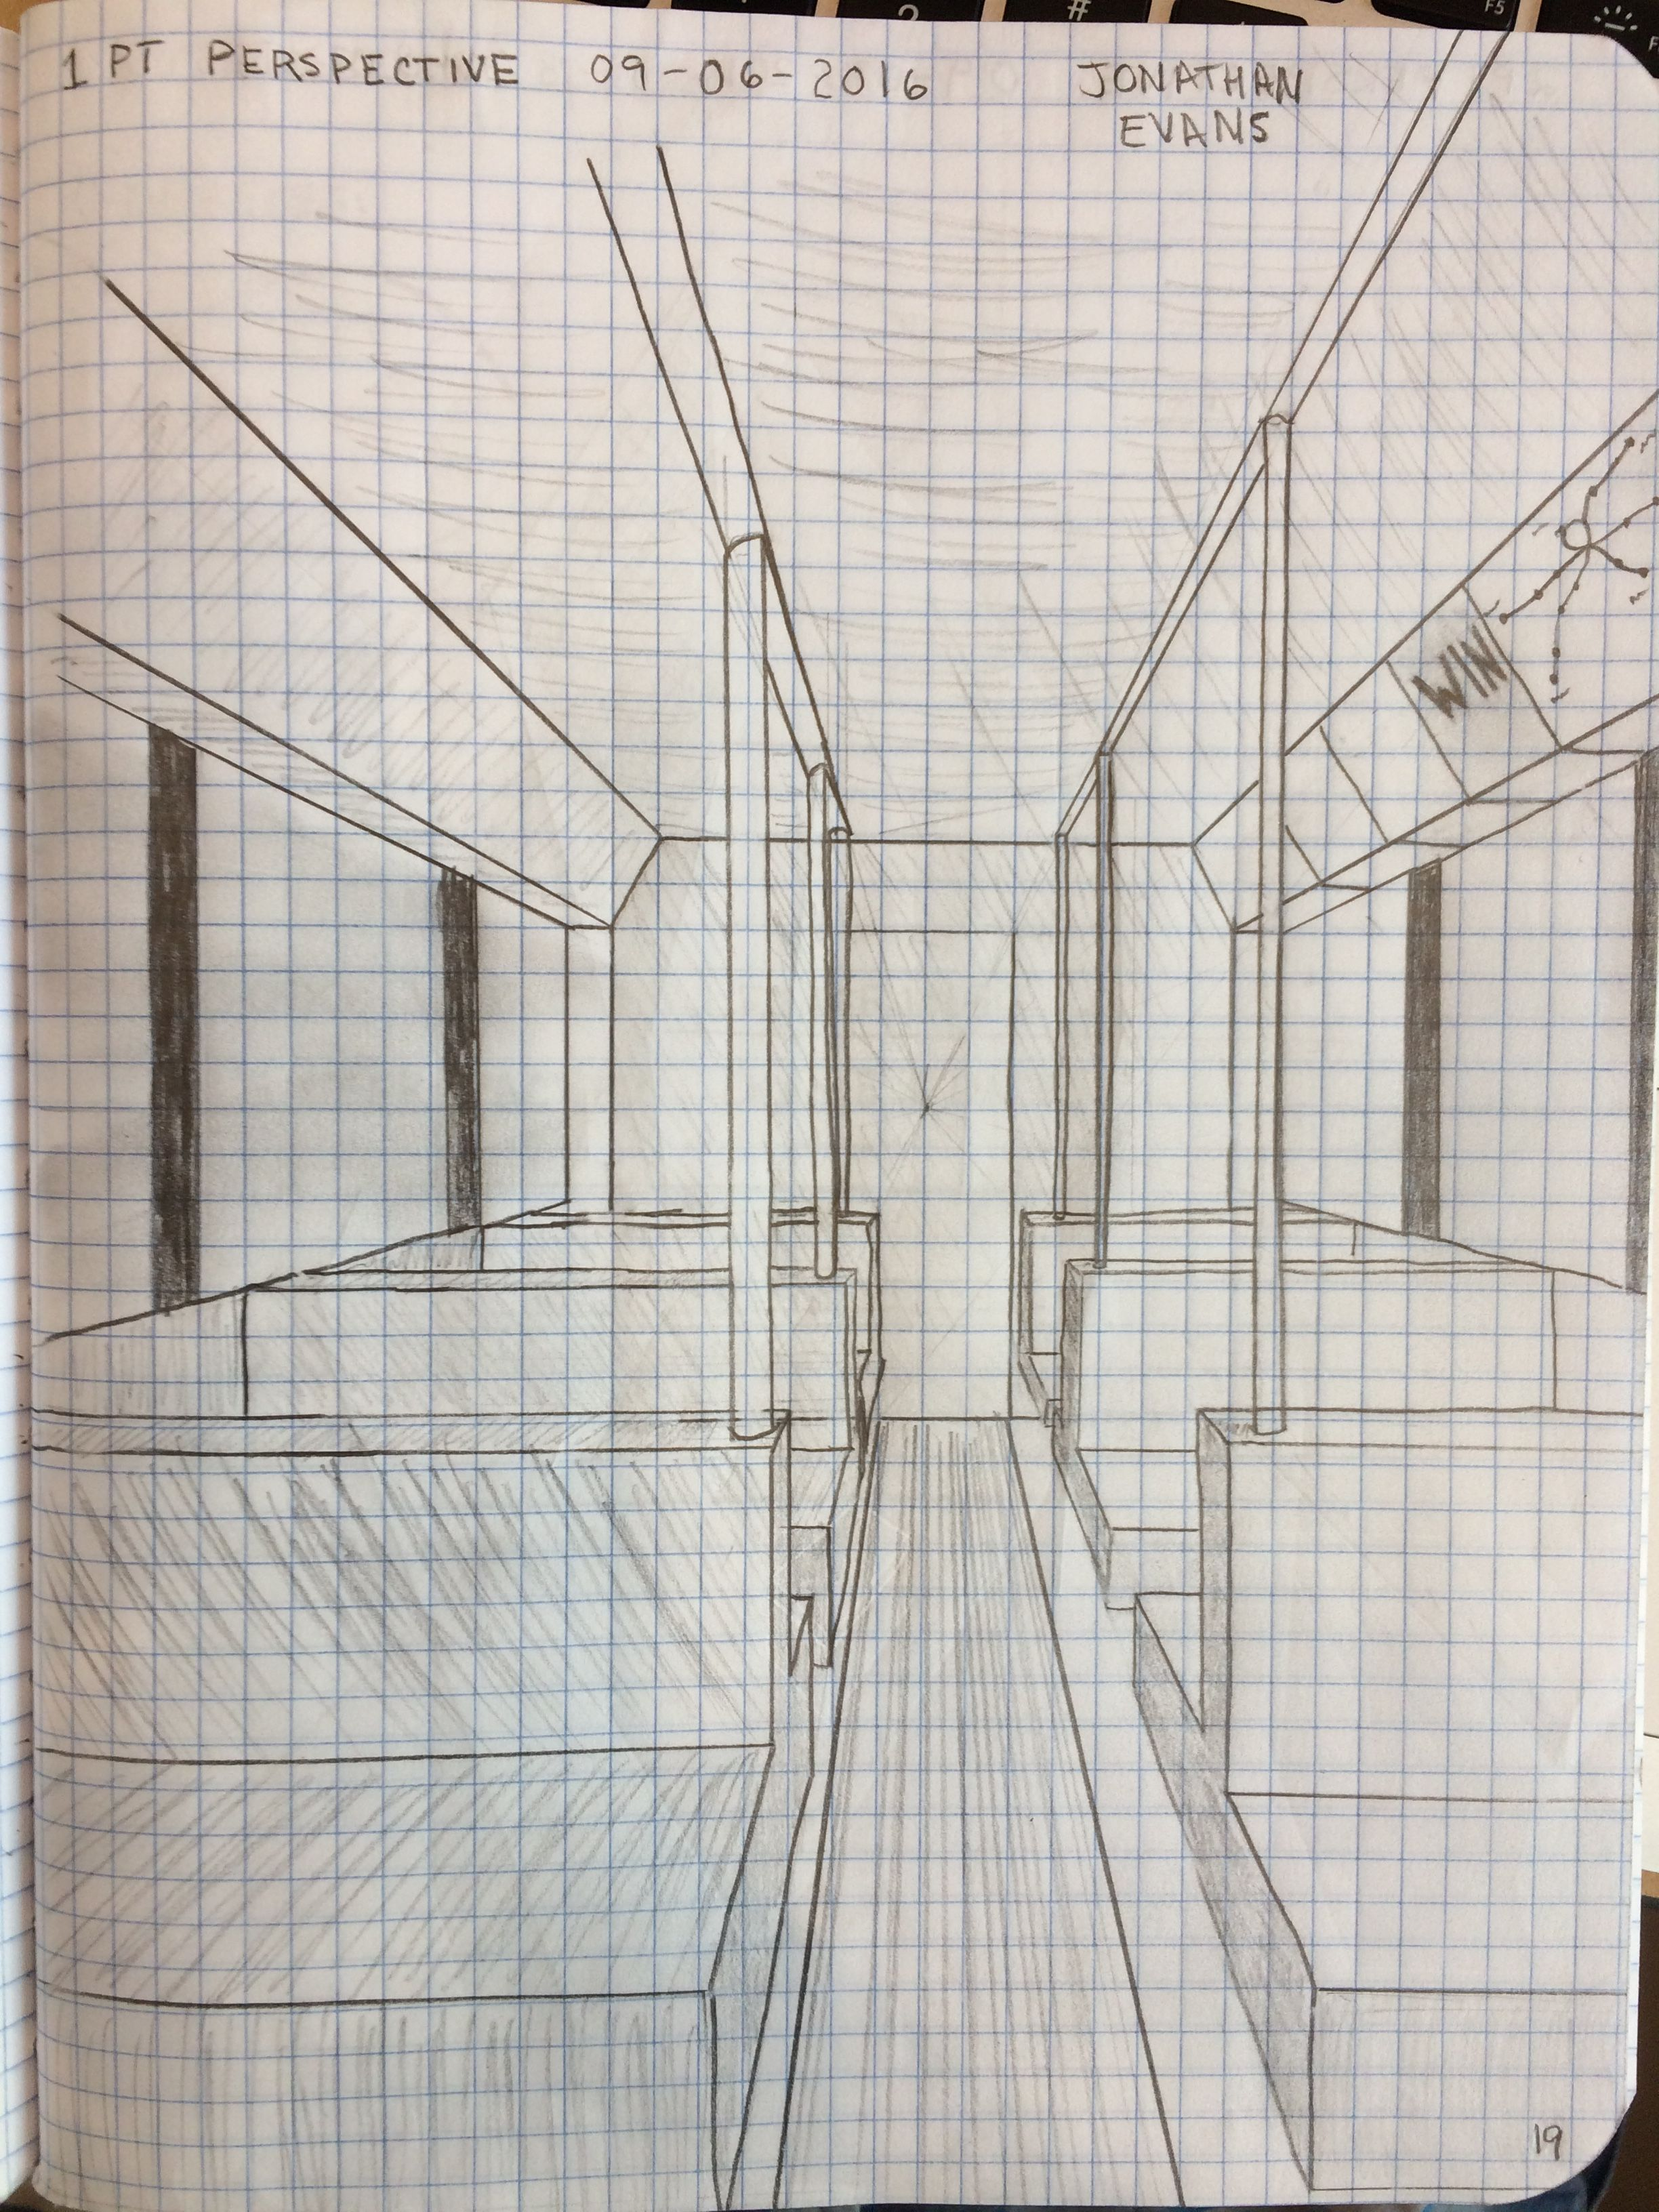
\includegraphics[width=160mm]{resources/light-rail-sketch.jpg}
%    \caption{Sketch of Inside of Light Rail}
%\end{figure}

\pagebreak

\begin{thebibliography}{9}
    \bibitem{cdc-food-deserts}
    Centers for Disease Control and Prevention (2012).
    \textit{A Look Inside Food Deserts} [Online].
    Available: \url{http://www.cdc.gov/features/FoodDeserts/index.html}.
    [Accessed 11 Sept. 2016].

    \bibitem{usda-food-deserts}
    United States Department of Agriculture Economic Research Service (2016).
    \textit{Food Access Research Atlas} [Online].
    Available:
    \url{http://www.ers.usda.gov/data-products/food-access-research-atlas/go-to-the-atlas.aspx}.
    [Accessed: 28 Oct. 2016].

\end{thebibliography}

\end{document}
